\chapter{Propuesta de solución}\label{chapter:Solution}

En este capítulo se ofrece la estructura general que representa la solución propuesta para codificar soluciones del VRP a un espacio continuo. Su diseño abstracto mediante dos componentes principales, \textit{encoder} y \textit{decoder}, permite la rápida adaptación de otra arquitectura de redes neuronales al modelo general. 

Como parte de la implementación se formularon dos modelos concretos para resolver el problema de codificación, \textit{\textbf{LinearAEC}} y \textit{\textbf{VAE}}. El primero de ellos está basado en un modelo \textit{autoencoder} clásico y el segundo, en un \textit{variational autoencoder}.

También se describe la etapa de generación y procesamiento de los datos para conformar los conjuntos de entrenamiento, prueba y validación. En este punto se retoman los tipos de representación vectorial de soluciones del VRP expuestos en la sección \ref{2-solS}.

A continuación se explica la idea central del problema, el procesamiento de los datos y el diseño de la solución. 


\section{Definición del problema}

La codificación de soluciones del VRP de un espacio discreto a vectores reales, surge por el interés de investigar el espacio continuo que puede obtenerse con el empleo de un modelo \textit{autoencoders} a partir de soluciones discretas del VRP.
De ahí que sea fundamental lograr una representación continua capaz de capturar sus características y propiedades.

El VRP es un problema de optimización combinatoria cuyo objetivo es minimizar el
 valor de una función de costo $C$ sobre el espacio $\mathcal{S}$ de soluciones, es decir $min \; C(s), \: s\in \mathcal{S}$ teniendo en cuenta las características y restricciones del problema. El espacio $\mathcal{S}$ lo forman soluciones representadas por vectores discretos, bien podrían ser cualquiera de las representaciones vistas en el capítulo \ref{chapter:REV-LL}. En este caso se considera que $\mathcal{S} \subset \mathbb{R}^{n}$, está formado por vectores con la misma estructura que los vectores $p$ analizados en \ref{2-Graph}.
 
 
 %En este caso $\mathcal{S}$ constituye un espacio de soluciones discretas del VRP, bien  y $\mathcal{S} \subset \mathbb{R}^{t}$ para algún $t$.
 
 La intención de este trabajo es obtener una representación $z \in \mathcal{Z}$ a partir de $s$, donde $\mathcal{Z}$ es un espacio continuo $\mathcal{Z} \subset \mathbb{R}^{l}$, para algún $l$. Es decir, determinar una función:
 \begin{equation}
 	f: \mathcal{S} \rightarrow \mathcal{Z},
 \end{equation}
 de forma tal que $f(s) = z$, y además, recuperar la solución codificada en $z$ mediante otra función:
  \begin{equation}
  g: \mathcal{Z} \rightarrow \mathcal{S},
  \end{equation}
 cuyo objetivo es conseguir que el resultado de $g(z) = s'$ sea lo más cercano posible a la entrada original $s$. Con esta idea, las soluciones iniciales $s$ se podrán representar mediante vectores con valores reales cuya dimensión depende de la dimensión del problema, y se conoce como código, vector de contexto o vector latente. 
 
Sea $s$ una solución del VRP, el problema enunciado puede reducirse a aproximar las funciones $f$ y $g$ de forma tal que $f(s) = z$ y $g(z) = s$ con el uso de técnicas de aprendizaje profundo, en particular: modelos \textit{autoencoders}. La funciones $f$ y $g$ se denominan \textit{encoder} y \textit{decoder} respectivamente y están constituidas por redes neuronales. La arquitectura específica del modelo se precisará en la sección \ref{3-GenStruct}, pero antes se describe el proceso seguido para generar los datos empleados en el proceso de entrenamiento.


\section{Procesamiento de datos de entrenamiento}\label{dataProc}

Una cuestión importante que se debe abordar antes de introducir el modelo es el procesamiento y preparación de los datos de entrada tal y como se señaló en \ref{1-etapas}. Como parte de esta etapa, se pueden aplicar varias técnicas que dependen del tipo de datos con los que se cuenta, por ejemplo si son de tipo texto o imagen. 

%En este caso se parte de la generación de soluciones del VRP representadas mediante los vectores $p$ explicados en \ref{2-Graph}, que luego se convierten a matrices 

El procesamiento previo permite una mejor adaptación entre los datos y la red neuronal mediante una serie de técnicas como vectorización de la información y normalización. Considerando que en la representación vectorial expuesta en \ref{2-Graph} con los vectores $p$, los valores no están normalizados, se decidió representar los datos a través de las matrices binarias $M$ analizadas en \ref{2-Matrix}. 

Como el objetivo principal es la codificación de una solución a un vector real, solo interesan en ellas, los clientes y cantidad $m$ de rutas. La conformación del conjunto de datos o soluciones iniciales para una instancia particular con $n$ clientes se desarrolló generando los vectores $p$, que como se había explicado, establecen la adyacencia en el grafo formado a partir de las rutas contenidas en la solución. Una vez obtenido ese conjunto de datos, cada solución del mismo se convierte a la matriz $M$ correspondiente, con el fin de obtener una representación normalizada.   

%Teniendo en cuenta las definiciones \ref{2-pi} y \ref{2-Matrix}, correspondientes a los vectores $p$ y las matrices binarias $M$ respectivamente, la transformación de un vector $p$ a una matriz $M$ se establece como sigue:


%Una instancia de un problema de enrutamiento de vehículos está definida por la cantidad de clientes $n$ y la cantidad de vehículos $m$. La conformación inicial del conjunto de datos para una instancia particular se desarrolló generando vectores $p$ que constituyen planificaciones de $m$ rutas para satisfacer los $n$ clientes. Luego de ello, se realiza una transformación sobre cada vector generado para obtener una  representación normalizada con matrices binarias.

%Sea $s \in \mathcal{S}$ una solución discreta a una instancia del VRP con $n$ clientes y $m$ vehículos, $p$ el vector de dimensión $n$ correspondiente según la interpretación ofrecida con grafos dirigidos, y $M$ la matriz binaria que se obtiene a partir de $p$. Primeramente se retoma la definición de ambas representaciones vectoriales:

%\[p[j]=\left\{
%\begin{array}{rcl}
%i & \mbox{si} & \text{el cliente $j + 1$ va detrás de $i + 1$ en la ruta. }\\
%&
%& \\
%j & \mbox{si} & \text{el cliente $j + 1$ es comienzo de ruta. }  \\
%&
%& \\
%\end{array}
%\right. \]


%\[M[i, j]=\left\{
%\begin{array}{rcl}
%1 & \mbox{si} & \text{el cliente $j + 1$ va detrás de $i + 1$ en la ruta.}\\
%&
%& \\
%1 & \mbox{si} & \text{$i = j$, la ruta está formada por un único cliente i + 1.}  \\
%&
%& \\
%0 & \mbox{eoc}  \\
%\end{array}
%\right. \]


%\[M[i, j]=\left\{
%\begin{array}{rcl}
%\label{Pi2M}
%1 & \mbox{si} & \text{$p[j] = i, \; i \neq j$}\\
%&
%& \\
%1 & \mbox{si} & \text{$p[j] = j, \; j + 1$ es el único cliente en su ruta}  \\
%&
%& \\
%0 & \mbox{eoc}  \\
%\end{array}
%\right. \]

%A continuación se muestra el procedimiento seguido para obtener $M$ a partir de $p$ mediante un ejemplo concreto. En particular se considerá el mismo vector de 9 clientes analizado en \ref{2-Graph}:
%\begin{center}
%	$p = [4, 1, 7, 5, 1, 5, 6, 6, 8],$
%\end{center}
%que se corresponde con la solución a través de listas de rutas:
%\begin{center}
%	$s = [(2, 5, 1), (6, 4), (7, 8, 3), (9)].$
%\end{center}

%Finalmente los pasos realizados se resumen en:
%\begin{eqnarray*}
%	p[0] = 4 \rightarrow  M[4, 0] = 1,\\
%	p[2] = 7 \rightarrow  M[7, 2] = 1,\\
%	p[3] = 5 \rightarrow  M[5, 3] = 1,\\
%	p[4] = 1 \rightarrow  M[1, 4] = 1,\\
%	p[7] = 6 \rightarrow  M[6, 7] = 1,\\
%	p[8] = 8 \rightarrow  M[8, 8] = 1, 
%\end{eqnarray*}

%El resto de las posiciones de $M$ tomarán valor 0 según la tercera condición de \ref{Pi2M}. Finalmente la matriz resultante es:

 %\begin{equation}
%\centering
%\begin{pmatrix}
%0 & 0 & 0 & 0 & 0 & 0 & 0 & 0 & 0\\
%0 & 0 & 0 & 0 & 1 & 0 & 0 & 0 & 0\\
%0 & 0 & 0 & 0 & 0 & 0 & 0 & 0 & 0\\
%0 & 0 & 0 & 0 & 0 & 0 & 0 & 0 & 0\\
%1 & 0 & 0 & 0 & 0 & 0 & 0 & 0 & 0\\
%0 & 0 & 0 & 1 & 0 & 0 & 0 & 0 & 0\\
%0 & 0 & 0 & 0 & 0 & 0 & 0 & 1 & 0\\
%0 & 0 & 1 & 0 & 0 & 0 & 0 & 0 & 0\\
%0 & 0 & 0 & 0 & 0 & 0 & 0 & 0 & 1\\
%\end{pmatrix}
%\end{equation}
%la cual coincide con la misma analizada en \ref{M9}.

%Dada la estructura y propiedades de este tipo de matrices, es fácil revertirlas para obtener la solución $s$ correspondiente. No obstante, como no se establece una biyección entre $s$ y $M$, la generación de los datos será mediante otro array que se nombrará como $pi$. 

Una vez representadas las soluciones del VRP como un vector donde cada componente pertenece al intervalo $[0, 1]$, se puede presentar la estructura general del modelo propuesto en la siguiente sección.

%Como se había mencionado, la solución implementada posee una estructura general a la cual se adaptaron los dos modelos propuestos, específicamente, evidenciada en el uso de sus dos componentes principales. En la siguiente sección se profundiza sobre esta cuestión. 


\section{Estructura general del modelo propuesto}\label{3-GenStruct}

El modelo ofrecido en este trabajo para la codificación de soluciones de un problema VRP, sigue la idea general de los modelos \textit{autoencoders} descritos en \ref{2-AEC} y consiste en dos componentes principales:  \textit{encoder} y \textit{decoder}. En la figura \ref{modelGeneral} se muestra un esquema general del modelo.

\begin{figure}[!h]
	\centering
	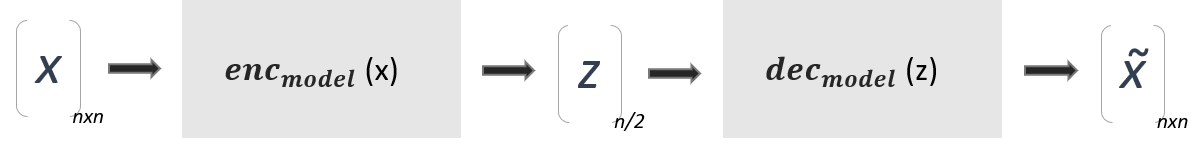
\includegraphics[width=5in]{Graphics/model general.png}
	
	\caption{ \small{Esquema general del modelo propuesto con las componentes \textit{encoder} y \textit{decoder}.}}
	
	\label{modelGeneral}
\end{figure}  

Dichas componentes son las encargadas de aproximar las funciones $f$ y $g$ mencionadas en la definición del problema, de foma tal que $f$ se reemplaza por la componente \textit{encoder} y $g$ se sustituye por la componente \textit{decoder}. Ambas están relacionadas mediante tres vectores que juegan un papel fundamental: el vector de entrada $x$, vector de contexto $z$ y el vector de salida $\tilde{x}$.

Los \textbf{vectores de entrada} constituyen matrices binarias de dimensión $n \times n$ representando a las soluciones del VRP. Además de ser la entrada a la red general, son la entrada de la componente \textit{encoder}. Este devuelve como salida un vector real denotado por $z$ que se conoce como \textbf{vector de contexto}. Posteriormente el \textit{decoder} procesa el vector $z$ y retorna un \textbf{vector de salida} que establece una reconstrucción de la entrada $s$. Tanto la entrada inicial al modelo como la salida final presentan las mismas dimensiones como se observa en el esquema \ref{modelGeneral}.

La configuración de parámetros en las componentes y la dimensión del vector $z$ dependen de la dimensión del problema, por tanto, la arquitectura del modelo se ajusta al tipo de problema particular. Debido a ello es necesario entrenar el modelo para cada dimensión del problema, o sea, para una cantidad de clientes fija.


\subsection{Funcionalidades del modelo propuesto}

La estructura genérica presentada anteriormente permite el uso de las componentes \textit{encoder} y \textit{decoder} de forma independiente, una vez que se entrene el modelo. En este sentido se distinguen tres funcionalidades que cumple el esquema general de la solución.

Siguiendo las definiciones señaladas en este capítulo, se denotará como $s$ el vector de entrada al modelo que representa una solución del VRP, $z$ el vector de contexto representativo de $s$ en el espacio continuo y $s'$ la reconstrucción de $s$ y también salida del modelo. A partir de este momento, las componentes \textit{encoder} y \textit{decoder} también serán tratadas como $enc_{model}$ y $dec_{model}$. 

Las funcionalidades referidas se exponen a continuación:

\begin{itemize}
	\item \textbf{codificar (encode)}: Mediante esta función es posible obtener el vector de código para una entrada $s$ cualquiera, de forma tal que:
	\begin{equation}
		encode(s) = enc_{model}(s) = z
	\end{equation}
	\item \textbf{decodificar (decode)}: A partir de un vector $z$ del espacio continuo, se puede producir la solución correspondiente en el espacio discreto aplicando:
	\begin{equation}
	decode(z) = dec_{model}(z) = s'
	\end{equation}
	
	\item \textbf{predecir (predict)}: Esta función da como resultado el vector reconstruido luego de atravesar por las dos etapas básicas de codificación y decodificación. Su empleo tiene sentido con el modelo ya entrenado para comprobar el desempeño del mismo. El funcionamiento consiste en:
	\begin{equation}
	predict(s) = dec_{model}(enc_{model}(s)) = s'
	\end{equation}
\end{itemize}

En la siguiente sección se profundizará en la descripción de ambos modelos, teniendo en cuenta la arquitectura de redes neuronales seleccionada.


\section{Modelos propuestos}

Como parte de la implementación de la propuesta de solución, se diseñaron dos modelos \textit{autoencoders} para intentar resolver el problema: \textit{\textbf{LinearAEC}} y \textit{\textbf{VAE}}. El primero de ellos conformado sobre la base de un \textit{autoencoders} clásico y el segundo, como su nombre lo indica, ideado a partir de un prototipo de VAE tradicional.

La función de pérdida de reconstrucción empleada en ambos modelos fue $MSE$ (Mean Squared Error), el promedio del cuadrado de las diferencias entre la entrada y la salida. La última capa de cada modelo utiliza la función de activación \textit{sigmoid}, y además, se decidió usar como optimizador \textit{RMSProp}, siguiendo las sugerencias brindadas en \textit{Chollet et al.} \cite{Chollet}. En el resto de las capas de ambos, se utiliza la función de activación \textit{relu}.

En lo adelante se denotarán como $E_i$ y $D_i$ las capas pertenecientes a las redes \textit{encoder} y \textit{decoder} respectivamente. Las características específicas, arquitectura y configuración de ambas propuestas serán abordadas en las siguientes secciones.
 

\subsection{Modelo \textit{LinearAEC}}\label{LinearAEC}

El carácter lineal de esta propuesta está determinado por la arquitectura de capas densas empleado. Tal y como se mencionó en \ref{3-GenStruct}, se encuentra conformado por dos componentes principales y tres vectores importantes. La configuración de la arquitectura y los parámetros correspondientes será detallada a continuación.

\subsubsection{Arquitectura del modelo}

Ambas componentes principales \textit{encoder} y \textit{decoder} constituyen redes neuronales formadas por capas densas. En la figura \ref{AECmodel} se muestra la estructura interna del modelo de inicio a fin:\\

\newpage

\begin{figure}[!h]
\centering
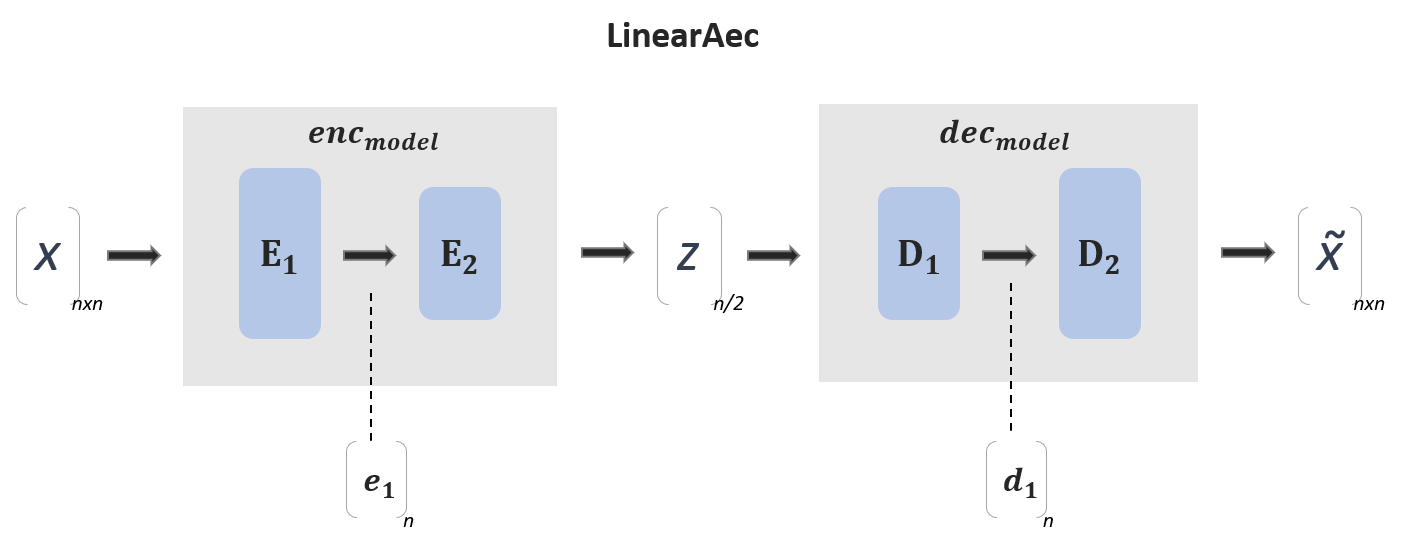
\includegraphics[width=5in]{Graphics/Aecmodel.png}

\caption{ \small{Diagrama del modelo LinearAEC}}

\label{AECmodel}
\end{figure}  


El \textit{encoder} recibe una matriz de entrada $x$ la cual se introduce a la primera capa oculta $E_1$. La salida de esta se conforma mediante la función de activación \textit{relu} y pasa a ser la entrada de la siguiente capa $E_2$, encargada de devolver el vector de contexto $z$. Durante la codificación, la dimensión de los vectores entre una capa y otra va disminuyendo hasta obtener $z$.

Posteriormente, $z$ se convierte en la entrada de la red \textit{decoder} donde será decodificado con el objetivo de recuperar la entrada $x$ inicial. La primera capa de entrada $D_1$ en esta componente, recibe el vector latente y devuelve como salida un vector de mayor dimensión con respecto a $z$, que será la entrada de la última capa $D_2$. Esta capa es la encargada de reconstruir la solución representada en $x$. Durante el proceso de decodificación la dimensión de los vectores de salida va incrementando en correspondencia con la disminución que se establece con la codificación. Por tal motivo, se puede decir que ambos procesos sin simétricos.





\subsection{Modelo \textit{VAE}}
Los VAE constituyen una versión más moderna de los \textit{autoencoders} que proporcionan una noción probabilística para describir un punto del espacio latente. En lugar de generar valores directamente para el estado latente como se hace en \ref{LinearAEC}, el modelo de codificación de un VAE generará parámetros que describen un distribución para cada dimensión en el espacio latente. Dado que se asume una distribución Normal, se generan dos vectores que describen la media y varianza de las distribuciones del espacio. Al generar puntos de tal distribución se obtienen nuevos datos, por eso es considerado un modelo generativo. Finalmente el \textit{decoder} procederá a desarrollar una reconstrucción de la entrada original. 

\subsubsection{Arquitectura del modelo} 


Similar al \textit{LinearAEC}, en el \textit{VAE}, las componentes \textit{encoder} y \textit{decoder} constituyen redes neuronales conformadas por capas densas. Lo interesante y diferente en este modelo, con respecto al \textit{LinearAEC}, es el proceso intermedio donde se genera el vector latente $z$. En la figura \ref{VAEmodel} se muestra un diagrama de la estructura interna del \textit{VAE} implementado, que facilitará la comprensión de sus etapas.\\


\begin{figure}[!h]
	\centering
	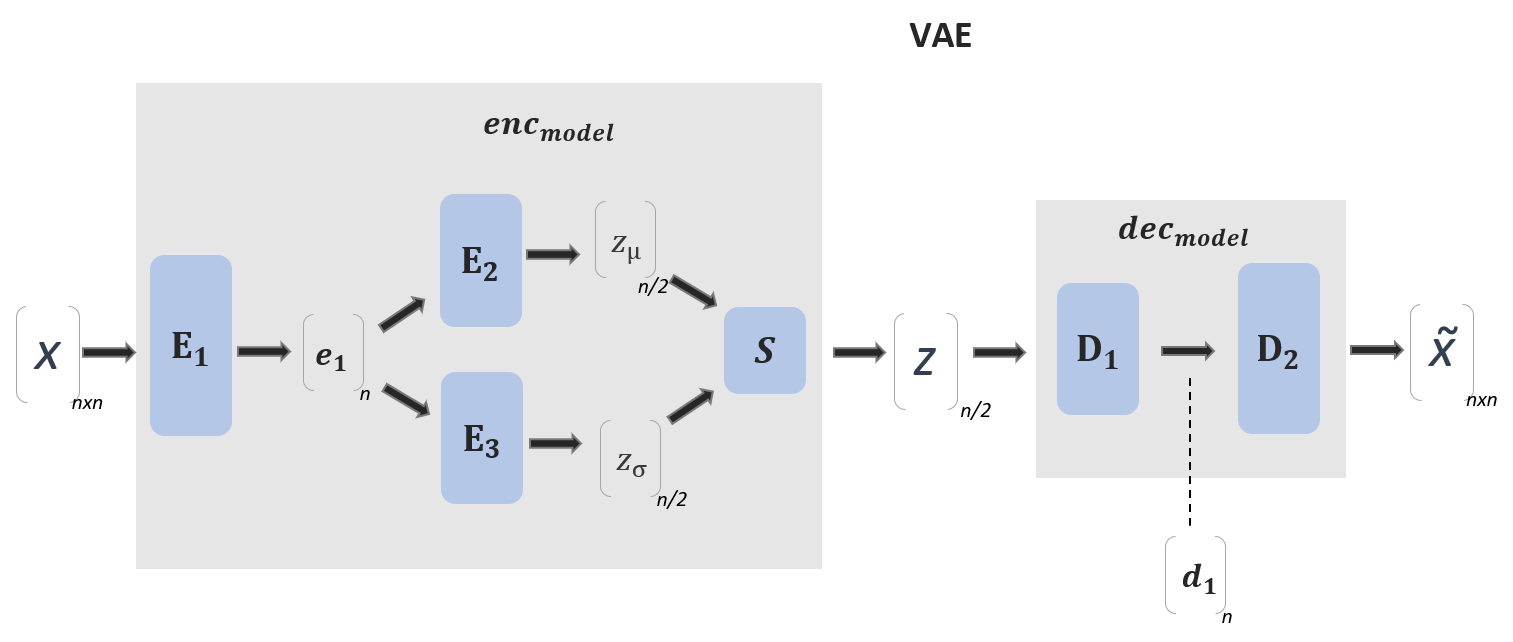
\includegraphics[width=5in]{Graphics/vaemodel.png}
	
	\caption{ \small{Diagrama del modelo VAE}}
	
	\label{VAEmodel}
\end{figure}  

El \textit{encoder} recibe un vector de entrada $x$ de dimensión $nxn$ el cual se procesa por la  capa de entrada $E_1$. A partir de este punto, es donde el proceso de codificación cambia en comparación con el \textit{LinearAEC}. Pues la salida de $E_1$ se introduce paralelamente a otras dos capas ocultas independientes que se identifican como $E_2$ y $E_3$.

El papel de estas nuevas capas es producir los vectores que describen la distribución de las codificaciones $z$. A través de $E_2$ se obtiene $z_{mean}$ y con $E_3$ se origina $z_{log {\_} sigma}$. Hasta el momento se ha explicado el punto número 1 de \ref{VAESteps}, donde se tiene que:

\begin{equation}
	z_{mean} , \; z_{log\_sigma} = enc_{model}(x)
\end{equation} 

Como parte de la generación del vector $z$ con los parámetros de la media y varianza de la distribución, se creó una capa personalizada que se denomina \textit{Sampling}. La capa se denota como $S$ en la figura \ref{VAEmodel}, recibe los parámetros mencionados y su esencia consiste en $	z = z_{mean} + exp(z_{log{\_}sigma})*\epsilon$. 

Una vez generado el vector $z$, este se convierte en la entrada del \textit{decoder}. En lo adelante, el comportamiento del \textit{decoder} es igual a la decodificación en el \text{LinearAEC}. Constituido por dos capas densas consecutivas $D_1$ y $D_2$, donde el vector de salida va aumentando de dimensión de una capa a la otra. Finalmente se obtiene la salida $\tilde{x}$ como reconstrucción de la entrada inicial $x$.\\

En el presente capítulo se expusieron dos modelos concretos para obtener una representación continua de las soluciones del VRP. Ambos se sustentan en la teoría analizada en el capítulo \ref{chapter:REV-LL} e intentan describir una distribución de probabilidad de los vectores de codificación. En el siguiente capítulo se muestran los resultados obtenidos a partir de dos escenarios donde se evalúa el comportamiento de los mismos.



 



